\graphicspath{{chapters/greco/images/level7/}}
\section{The Properties of the GRECO Event Selection}
The completion of cuts yields the completed GRECO event selection.
The rates of each sample of simulation and data are shown numerically in \ref{tab:event_rates} or graphically in \ref{fig:event_rates}.
Also included is the analysis binning as described in \ref{subsec:binning} for reference.

\begin{table}[]
\centering
\begin{tabular}{@{}lllllllll@{}}
\toprule
Type              & \multicolumn{3}{l}{IceCube Processing}     & \multicolumn{4}{l}{GRECO}             & Analysis         \\ 
                     & Any Filter   & DC Filter  & Low-en L3        & L4         & L5       & L6    & L7          & Binning \\ \midrule
CORSIKA        & 990598     & 9178      & 969.818           & 50.511  & 4.100  & 0.443 & 0.100   & 0.092            \\
MuonGun        & 60669       & 2982      & 442.493          & 33.562  & 3.022   & 0.315 & 0.080   & 0.07             \\
Accidentals    & 35855       & 8117      & 283.559           & 11.963  & 1.799  & 0.102 & 0.002   & 0.001            \\
$\nu_e$        & 1.842        & 1.721     & 1.262               & 0.783    & 0.544  & 0.362 & 0.325   & 0.194            \\
$\nu_{\mu}$ & 11.317      & 6.360     & 4.758               & 2.503    & 1.629  & 1.011 & 0.676   & 0.552            \\
$\nu_{\tau}$ & 0.293        & 0.270     & 0.206              & 0.134    & 0.103  & 0.074 & 0.051   & 0.045            \\ \midrule
MC Total*       & 1026466   & 17303    & 1260               & 65.893  & 8.176  & 1.991 & 1.153   & 0.884            \\
Data              & 1154426   & 19092    & 1092               & 68.592   & 7.422  & 1.841 & 0.871   & 0.715            \\ \bottomrule
\end{tabular}
\caption{The event rates at each cut level in the GRECO selection. Note that the MuonGun events are included in this table, but do not contribute to the total Monte Carlo expectation to prevent double-counting of muon events from the CORSIKA sample. All rates are given in millihertz.}
\label{tab:event_rates}
\end{table}


\label{subsubsec:greco_truth}
\subsection{Energy and Zenith Reach}
The GRECO sample covers a wide range of energies, with some final level events possessing energies as low as 2 GeV or as high as 1 TeV.
The bulk of the neutrino sample, shown in \ref{fig:true_nuproperties}, occurs at the expected oscillation minimum near 25 GeV.
Most neutrino events originate at the horizon, as expected from the atmospheric neutrino flux, although there exists an asymmetry between the upward- and downward-going events.
This asymmetry originates from the event selection, which selects against downward-going events in order to minimize the atmospheric muon background.

\begin{center}
\begin{table}
\begin{tabular}{cc}
	\label{fig:gev_per_nch} 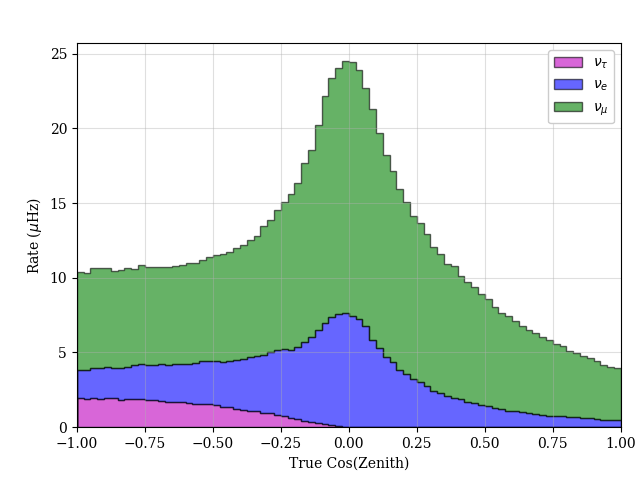
\includegraphics[width=0.45\linewidth]{L7_true_coszen.png} &
	\label{fig:t_rms} 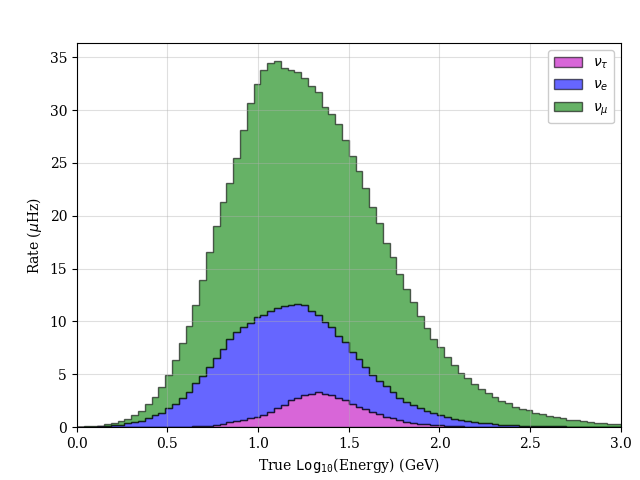
\includegraphics[width=0.45\linewidth]{L7_true_logen.png} \\
\end{tabular}
\label{fig:true_nuproperties}
\caption{The true neutrino energy and zenith of the GRECO sample at final level. The sample shows an asymmetry between upgoing ($\mathtt{cos(\theta)<0}$) and downgoing ($\mathtt{cos(\theta)>0}$) event rates in the neutrinos due to selection bias. The sample has a long tail of events at both high and low energies. Using the NuFit 2.2 oscillation parameters and the flux model from Honda, the $\mathtt{\nu_\tau}$ events are observed in the very upgoing region around $\mathtt{10^1.4=25}$ GeV. }
\end{table}
\end{center}

\label{subsubsec:greco_reco}
\subsection{Reconstructed Variables}
The true variables of the neutrino distributions are not observables in most GRECO analyses.
Instead, all events are described using the reconstructed energies and zenith angles.
The $\mathtt{\nu_\tau}$ sample reconstructs to slightly lower energies due to the loss in energy from the outgoing neutrino.
The sample, when compared to data, shows reasonable shape agreement in both energy and zenith, although systematic disagreements occur above 100 GeV.

\begin{center}
\begin{table}
\begin{tabular}{cc}
	\label{fig:gev_per_nch} 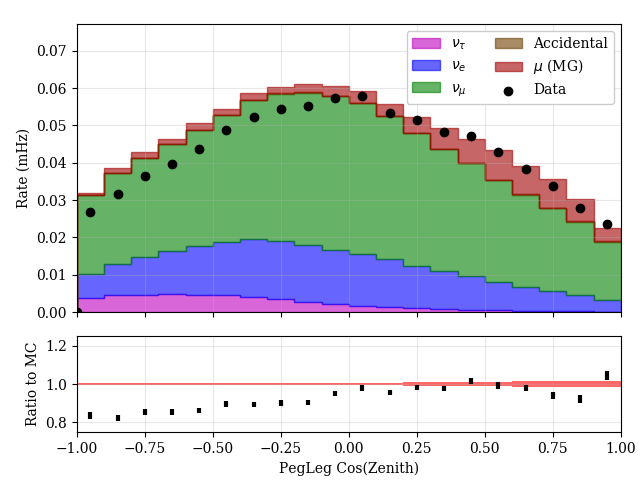
\includegraphics[width=0.45\linewidth]{L7_reco_coszen.png} &
	\label{fig:t_rms} 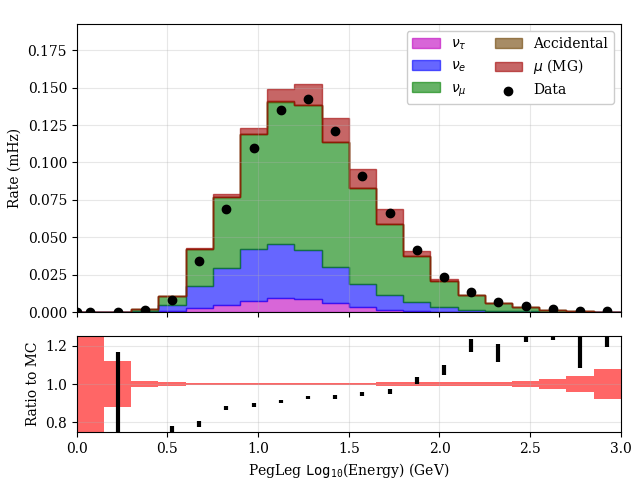
\includegraphics[width=0.45\linewidth]{L7_reco_logen.png} \\
\end{tabular}
\label{fig:true_nuproperties}
\caption{The reconstructed energy and zenith of the GRECO sample at final level. Events in data reconstruct to both relatively high energies ($\mathtt{E_{R}>100}$ GeV) and very low energies ($\mathtt{E_{R}\approx2}$ GeV). Using the NuFit 2.2 oscillation parameters and the flux model from Honda, the $\mathtt{\nu_\tau}$ events are observed in the very upgoing region around $\mathtt{10^1.4=25}$ GeV. }
\end{table}
\end{center}